Bevor damit begonnen werden kann \"uberhaupt eine Gruppenstruktur auf \(\Theta_n\) zu definieren, m\"ussen zun\"achst einige Vorbereitungen getroffen werden. Im Folgenden seien alle Mannigfaltigkeiten, soweit nicht anders spezifiziert, zweit\-ab\-z\"ahl\-bar, kompakt und glatt (m\"oglicherweise mit Rand). Die Annahme der Glattheit ist keine Einschr\"ankung gegen\"uber der \(\mathcal{C}^k\)-Differenzierbarkeit, da zu jeder differenzierbaren Mannigfaltigkeit mit einer \(\mathcal{C}^k\)-Struktur \(\mathfrak{A}\) eine \(\mathcal{C}^{\infty}\)-Struktur \(\mathfrak{B}\) und ein \(\mathcal{C}^k\)-Diffeomorphismus \((\mathcal{M},\mathfrak{A})\to(\mathcal{M},\mathfrak{B})\) existiert \cite{hirsch2012difftop} Satz 3.4. Eine kompakte Mannigfaltigkeit mit leerem Rand hei\ss e \textbf{geschlossen}. 

\section{Orientierbarkeit und Poincar\'e-Dualit\"at}
    Sei \(\mathcal{M}^n\) eine kompakte, topologische Mannigfaltigkeit. Ist diese geschlossen, ist sie genau dann orientierbar, wenn \(H_n(\mathcal{M})\cong\mathbb{Z}\) gilt. Ist sie berandet, muss \(H_n(\mathcal{M},\partial\mathcal{M})\cong\mathbb{Z}\) gelten. Eine Wahl eines Erzeugers dieser Gruppen korrespondiert mit der Wahl einer Orientierung von \(\mathcal{M}\), hei\ss e \textbf{Fundamentalklasse} von \(\mathcal{M}\) und wird gelegentlich unter leichtem Notationsmissbrauch mit \(\eqcl{\mathcal{M}}\) bezeichnet. Ist \(\mathcal{M}\) nicht zusammenh\"angend, sei eine Orientierung eine Wahl von Fundamentalklassen aller Komponenten. Im Folgenden werden alle Mannigfaltigkeit als orientierbar angenommen. Wenn \(\iota\colon\mathcal{M}\hookrightarrow\mathcal{W}\) eine Einbettung ist, kann \(\eqcl{\mathcal{M}}\) als Element von \(H_n(\mathcal{W})\) aufgefasst werden. Schreibe f\"ur die inkludierte Homologieklasse
\[\eqcl{\mathcal{M}\mathrel{|}\mathcal{W}}:=\iota_*\eqcl{\mathcal{M}}\in H_n(\mathcal{W})\,.\]
Ist \(\mathcal{M}\) geschlossen, sagt die \textbf{Poincar\'e-Dualit\"at} nun gerade aus, dass der Homomorphismus 
\[H^k(\mathcal{M})\to H_{n-k}(\mathcal{M}),\,p\mapsto p\frown\eqcl{\mathcal{M}}\]
ein Isomorphismus ist (\cite{hatcher2002algebraic} Satz 3.30). Ist der Rand nicht leer, nimmt diese Isomorphie die Formen
\[H^k(\mathcal{M})\mathop{\cong}H_{n-k}(\mathcal{M},\partial\mathcal{M})\quad\text{und}\quad H^k(\mathcal{M},\partial\mathcal{M})\mathop{\cong}H_{n-k}(\mathcal{M})\]
an. Im Folgenden sei das duale Element von \(x\) auch durch \(x^*\) gekennzeichnet. Ist \(\mathcal{W}^n\) ein Kobordismus mit \(\partial\mathcal{W}\cong\partial_-\mathcal{W}\sqcup\partial_+\mathcal{W}\). Dann gilt die \textbf{Lefschetz-Dualit\"at}, also ist 
\[H^k(\mathcal{W},\partial_-\mathcal{W})\to H_{n-k}(\mathcal{W},\partial_+\mathcal{W}),\,\sigma\mapsto\sigma\frown\eqcl{\mathcal{W}}\,.\]
ist ein Isomorphismus (\cite{hatcher2002algebraic} Satz 3.43). Die langen exakten Folgen der Homomologie und der Kohomologie sind dabei durch folgendes bis auf Vorzeichen kommutative Diagramm verbunden (\cite{dold1980lectures} Abschnitt VIII Satz 9.1), in welchem \(i+j=n\) gelte.
\begin{equation}\label{diag:poin_exact}
    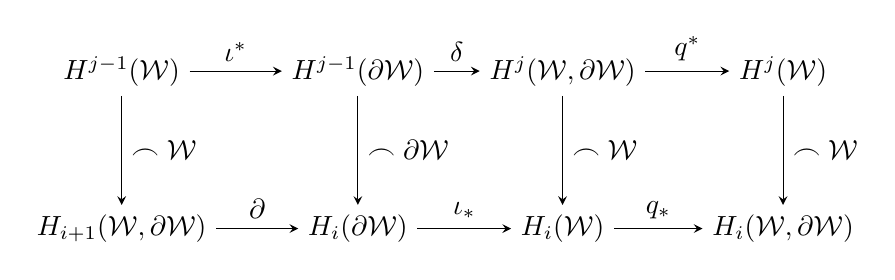
\begin{tikzpicture}[baseline=(current  bounding  box.center)]
        \draw 
            (0, 0) node (A) {\(H_{i+1}(\mathcal{W},\partial\mathcal{W})\)}
            (3, 0) node (B) {\(H_i(\partial\mathcal{W})\)}
            (5.6, 0) node (C) {\(H_i(\mathcal{W})\)}
            (8.4, 0) node (D) {\(H_i(\mathcal{W},\partial\mathcal{W})\)}
            (0, 2) node (E) {\(H^{j-1}(\mathcal{W})\)}
            (3, 2) node (F) {\(H^{j-1}(\partial\mathcal{W})\)}
            (5.6, 2) node (G) {\(H^j(\mathcal{W},\partial\mathcal{W})\)}
            (8.4, 2) node (H) {\(H^j(\mathcal{W})\)}
            (A) edge [-stealth] node [above] {\(\partial\)} (B)
            (B) edge [-stealth] node [above] {\(\iota_*\)} (C)
            (C) edge [-stealth] node [above] {\(q_*\)} (D)
            (E) edge [-stealth] node [above] {\(\iota^*\)} (F)
            (F) edge [-stealth] node [above] {\(\delta\)} (G)
            (G) edge [-stealth] node [above] {\(q^*\)} (H)
            (E) edge [-stealth] node [right] {\(\frown\eqcl{\mathcal{W}}\)} (A)
            (F) edge [-stealth] node [right] {\(\frown\eqcl{\partial\mathcal{W}}\)} (B)
            (G) edge [-stealth] node [right] {\(\frown\eqcl{\mathcal{W}}\)} (C)
            (H) edge [-stealth] node [right] {\(\frown\eqcl{\mathcal{W}}\)} (D)
            ;
    \end{tikzpicture}
\end{equation}
    
\section{Die Schnittpaarung}
    Sei \(\mathcal{W}^n\) eine Mannigfaltigkeit und \(i+j=n\). Dann l\"asst sich \"uber die Kronecker-Paarung und Poincar\'e-Dualit\"at eine Bilinearform
\[\mathrel{-}\cdot\mathrel{-}\,\colon H_i(\mathcal{W})\otimes H_j(\mathcal{W})\to\mathbb{Z},\,x\cdot y:=\left\langle x^*\smile y^*,\eqcl{\mathcal{W}}\right\rangle\]
definieren. Aus den Eigenschaften des Cup-Produktes folgt einerseits
\begin{equation}\label{eq:intersect_prop_1}
    x\cdot y=\left\langle x^*\smile y^*,\eqcl{\mathcal{W}}\right\rangle=(-1)^{ij}\left\langle y^*\smile x^*,\eqcl{\mathcal{W}}\right\rangle=(-1)^{ij}(y\cdot x)\,,
\end{equation}
aus den Eigenschaften der Kroneckerpaarung ergibt sich
\begin{equation}\label{eq:intersect_prop_2}
    x\cdot y=\langle x^*\smile y^*,\eqcl{\mathcal{W}}\rangle=\langle q^*x^*,y^*\frown\eqcl{\mathcal{W}}\rangle=\langle q^*x^*,y\rangle\,.
\end{equation}
Da \(\mathcal{M}\) eine orientierbare Mannigfaltigkeit ist, besitzt die Auswertungsabbildung eine besonders einfache Form. Es gilt:
\begin{lemma}\label{lem:intersect_factor}
    Die Abbildung \({\operatorname{Ad}\colon H_i(\mathcal{M})\to\operatorname{Hom}(H_j(\mathcal{M}),\mathbb{Z}),\,x\mapsto x\cdot(\mathrel{-})}\) ist gleich der Komposition
    \[H_i(\mathcal{M})\mathop{\longrightarrow}^{q_*}H_i(\mathcal{M},\partial\mathcal{M})\mathop{\longrightarrow}^{\text{\tiny P.D.}}H^j(\mathcal{M})\mathop{\longrightarrow}^{\text{\tiny U.K.}}\operatorname{Hom}(H_j(\mathcal{M}),\mathbb{Z})\,.\]
\end{lemma}
\begin{proof}
    Die Komposition bildet \({x\in H_i(\mathcal{M})}\) auf \({\langle\left(q_*(x)\right)^*,\mathrel{-}\rangle}\) ab, wobei aus Diagramm \ref{diag:poin_exact} folgt, dass die Gleichung \({(q_*(x))^*=q^*x^*}\) gilt. Dies zeigt
    \[\langle(q_*(x))^*,\mathrel{-}\rangle=\langle q^*x^*,\mathrel{-}\rangle\mathop{=}^{\text{\tiny\eqref{eq:intersect_prop_2}}}x\cdot(\mathrel{-})=\operatorname{Ad}(x)\,.\]
\end{proof}
\newpage
\begin{corollary}\label{crl:intersect_uni}
    Sei \(\mathcal{M}^{i+j}\) derart, dass \({H_i(\partial\mathcal{M})=H_{i-1}(\partial\mathcal{M})=0}\) gilt und \(H_{j-1}(\mathcal{M})\) frei ist. Dann ist \(\mathrel{-}\cdot\mathrel{-}\) unimodular.
\end{corollary}
\begin{proof}
    Betrachte die Faktorisierung
    \[\operatorname{Ad}\colon H_i(\mathcal{M})\mathop{\longrightarrow}^{q_*}H_i(\mathcal{M},\partial\mathcal{M})\mathop{\longrightarrow}^{\text{\tiny P.D.}}H^j(\mathcal{M})\mathop{\longrightarrow}^{\text{\tiny U.K.}}\operatorname{Hom}(H_j(\mathcal{M}),\mathbb{Z})\]
    gem\"a\ss{} Lemma \ref{lem:intersect_factor}. Aus den Annahmen folgt, dass alle Abbildungen isomorphismen sind.
\end{proof}
Die derart definierte Schnittform ist besonders interessant, wenn \(\mathcal{M}\) gerade Dimension besitzt und \(i=j\) gilt. In diesem Fall hei\ss e die Bilinearform \textbf{Schnittform}.
\commend{
    Seien \(\mathcal{M}\) und \(\mathcal{N}\) Untermannigfaltigkeiten komplement\"arer Dimension in \(\mathcal{W}\). Definiere ihre \textbf{Schnittzahl} durch
    \[\mathcal{M}\cdot\mathcal{N}:=\eqcl{\mathcal{M}\mathrel{|}\mathcal{W}}\cdot\eqcl{\mathcal{N}\mathrel{|}\mathcal{W}}\,.\]
    Diese Definition l\"asst sich geometrisch interpretieren. Ohne die Isotopieklasse von \(\mathcal{M}\) oder \(\mathcal{N}\) zu ver\"andern, kann angenommen werden, dass sich die beiden Mannigfaltigkeiten transversal schneiden. In diesem Fall ist \(\mathcal{V}:=\mathcal{M}\cap\mathcal{N}\) eine nulldimensionale Mannigfaltigkeit, die folglich aus endlich vielen Punkten besteht. In jedem Punkt \(p\in\mathcal{V}\) existiert nun aufgrund der Transversalit\"at eine direkte Summenzerlegung \(T_p\mathcal{W}=T_p\mathcal{M}\oplus T_p\mathcal{N}\). Eine positiv orientierte Basis von \(T_p\mathcal{M}\) zusammen mit einer positiv orientierten Basis von \(\mathcal{N}\) ergibt eine Basis von \(T_p\mathcal{W}\). Setze \(\epsilon_p:=1\), falls die zusammengesetzte Basis erneut positiv orientiert, und \(\epsilon_p:=-1\) sonst. Dann gilt
    \[\mathcal{M}\cdot\mathcal{N}\mathop{=\sum\epsilon_p}_{p\in\mathcal{M}\cap\mathcal{N}}\,.\]
    Dies folgt, da f\"ur transversale Mannigfaltigkeiten \(\mathcal{M}\) und \(\mathcal{N}\) die Identit\"at
    \[\eqcl{\mathcal{M}\cap\mathcal{N}\mathrel{|}\mathcal{W}}^*=\eqcl{\mathcal{M}\mathrel{|}\mathcal{W}}^*\smile\eqcl{\mathcal{N}\mathrel{|}\mathcal{W}}^*\in H^n(\mathcal{W})\]
    gilt, und eine Orientierung einer nulldimensionalen Mannigfaltigkeit \(\mathcal{V}\) gerade eine Wahl von \(\pm1\) f\"ur jeden Punkt \(p\in\mathcal{V}\) ist [REF].
}

\section{Immersionen und Whitneys Trick}
    Sei \(f\colon\mathcal{M}\looparrowright\mathcal{N}\) eine Immersion. Dann faktorisiert \(\dx f\) durch die kanonische Abbildung \(f^*T\mathcal{N}\to T\mathcal{N}\) und es existiert ein kommutatives Diagramm
\begin{center}
    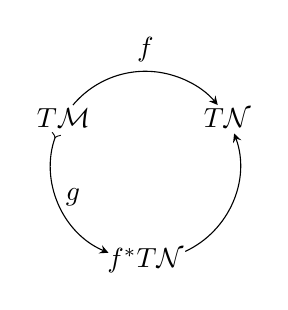
\begin{tikzpicture}[scale = 0.8]
        \draw
            (30:1.5) node (A) {\(T\mathcal{N}\)}
            (150:1.5) node (B) {\(T\mathcal{M}\)}
            (270:1.5) node (C) {\(f^*T\mathcal{N}\)}
            ;
            \draw [-stealth] (140:1.5) arc (140:40:1.5) node [pos = 0.5, above] {\(\dx f\)};
            \draw [>-stealth] (160:1.5) arc (160:247:1.5) node [pos = 0.45, right] {\(g\)};
            \draw [-stealth] (295:1.5) arc (295:380:1.5);
    \end{tikzpicture}
\end{center}
sodass sich das Normalenb\"undel von \(f\) als \(\nu(f):=f^*T\mathcal{N}/g(T\mathcal{M})\) definieren l\"asst. Ist \(f\) eine Einbettung, entspricht dies gerade dem bekannten Normalenb\"undel. Analog zu der Schnittzahl zweier transversaler Mannigfaltigkeiten kann die Selbstschnittzahl einer Immersion \(f\colon\mathcal{M}^k\looparrowright\mathcal{N}^{2k}\) definiert werden. Es kann zun\"achst angenommen werden, dass \(f\) sich selbst transversal schneide und lediglich endlich viele Doppelpunkte \(f(p)=f(q)\) besitzt. Definiere \(\epsilon_p\) als \(1\), wenn die zusammengesetzte Orientierung von 
\[T_p\mathcal{N}=\dx_pf\left(T_p\mathbb{S}^k\right)\oplus\dx_qf\left(T_q\mathbb{S}^k\right)\]
der gew\"ahlten Orientierung von \(\mathcal{N}\) entspricht und \(-1\) sonst. Ist \(k\) gerade ist, sei die Selbstschnittzahl
\[I_f\mathop{:=\sum\epsilon_p}_{f(p)=f(q)}\,,\]
ist \(k\) ungerade sei sie eben jene Summe modulo zwei. Besonders wichtig ist diese Zahl in der Verwendung des starken Einbettungssatzes von Whitney, also auch in Whitneys Trick. Siehe Abbildung \ref{fig:whitney_trick}.

\begin{proposition}[Whitneys Trick]\label{prop:whit_trick}
    Sei \(k\geq3\), \(\mathcal{N}^{2k}\) einfach zu\-sam\-men\-h\"an\-gend und \(f\colon\mathcal{M}^k\looparrowright\mathcal{N}\) eine Immersion. \"Ubersteigt die Anzahl der Doppelpunkte von \(f\) die Zahl \(\abs{I_f}\), oder ist \(>0\) f\"ur ungerade \(k\), existiert eine regul\"ar homotope Immersion \(g\), die zwei Doppelpunkte weniger besitzt.
\end{proposition}
\begin{proof}
    Siehe \cite{whitney1944intersect} Satz 4.
\end{proof}

\begin{figure}
    \centering
    \begin{tikzpicture}
        \begin{scope}[xshift = -3cm]
            \draw 
                (2, 0) arc (10:170:2 and 1) 
                    node (A) [pos = 0.2] {\tiny\textbullet}
                    node (B) [pos = 0.8] {\tiny\textbullet}
                    node (C) [pos = 0.45] {}
                (2, 1) arc (-10:-170:2 and 1)
                    node (D) [pos = 0.55] {}
                (C.center) edge [densely dotted, -stealth] ++(0, -1.2)
                (D.center) edge [densely dotted, -stealth] ++(0, 1.2)
                ;
            \draw 
                (A) node [above] {\tiny\(q\)} node [below] {\tiny\(1\)}
                (B) node [above] {\tiny\(p\)} node [below] {\tiny\(-1\)}
            ;

            \fill [pattern = north west lines] 
                (A) arc (42:138:2 and 1) arc (-138:-42: 2 and 1) -- cycle;
        \end{scope}
        \draw (-0.75, 0.5) edge [-stealth] (0.75, 0.5);
        \begin{scope}[xshift = 3cm]
            \draw 
                (2, 0) arc (10:170:2 and 0.5) 
                    node (E) [pos = 0.45] {}
                (2, 1) arc (-10:-170:2 and 0.5)
                    node (F) [pos = 0.55] {}
                (E.center) edge [densely dotted, -stealth] ++(0, -0.75)
                (F.center) edge [densely dotted, -stealth] ++(0, 0.75)
                ;
        \end{scope}
    \end{tikzpicture}
    \caption{Die Idee von Whitneys Trick zur Eliminierung der Doppelpunkte \(p\) und \(q\) einer Immersion \(f\colon\mathbb{S}^1\looparrowright\mathcal{N}\). Der einfache Zusammenhang von \(\mathcal{N}\) garantiert, dass der schraffierte Bereich kontrahierbar ist.}\label{fig:whitney_trick}
\end{figure}

\begin{corollary}\label{cor:imm_reg_hom}
    Sei \(k\geq3\) ungerade, \(\mathcal{N}^{2k}\) einfach zusammenh\"angend und \(f\colon\mathcal{M}^k\looparrowright\mathcal{N}^{2k}\) eine Immersion. Die Selbstschnittzahl von \(f\) ist genau dann null, wenn \(f\) regul\"ar homotop zu einer Einbettung ist.
\end{corollary}

\begin{proposition}\label{prop:imm_inter_zero}
    Es existiert eine Immersion \(h\colon\mathbb{S}^k\looparrowright\mathbb{R}^{2k}\) mit Selbstschnittzahl eins.
\end{proposition}
\begin{proof}
    Siehe \cite{whitney1944intersect} Satz 3.
\end{proof}

\begin{figure}[!h]
    \centering
    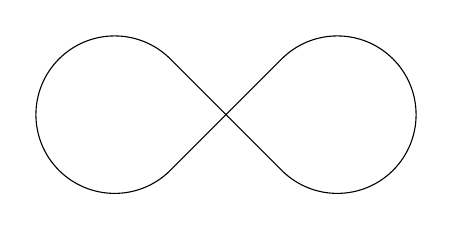
\begin{tikzpicture}
        \draw (-0.707, 0.707) arc (45:315:1) -- (0.707, 0.707) arc (135:-135:1) -- cycle;
    \end{tikzpicture}
    \caption{Eine Immersion \(f\colon\mathbb{S}^1\looparrowright\mathbb{R}^2\) mit Selbstschnittzahl eins.}\label{fig:double_imm}
\end{figure}


